%%This is a very basic article template.
%%There is just one section and two subsections.
\documentclass[a4paper, ngerman]{scrartcl}

\usepackage[T1]{fontenc}
\usepackage[utf8]{inputenc}
\usepackage[ngerman]{babel}
\usepackage{lmodern}
\usepackage{amsmath}
\usepackage{amsfonts}
\usepackage{hyperref}
\usepackage{graphicx}
\usepackage{paralist}
\usepackage[none]{hyphenat}
\usepackage{wrapfig}
\usepackage{subfig}
\usepackage{subfloat}

\def\sectionautorefname{Abschnitt}
\def\figureautorefname{Abbildung}

\sloppy



\hypersetup{
pdfborder = {0 0 0},
urlbordercolor = {0 0 0},
colorlinks = true,
linkcolor = black,
citecolor = black,
filecolor = black,
urlcolor  = black
}

\captionsetup[figure]{skip=5pt}

\title{Software-Challenge 2014 - Sixpack}
\subtitle{Spielregeln}



%% Variablen
\newcommand{\SpielFelderAnzahl}{\emph{256}}
\newcommand{\KartenAnzahl}{\emph{KartenAnzahl}}
\newcommand{\PiratenAnzahl}{\emph{6}}
\newcommand{\EmptyPlainPage}{\newpage\thispagestyle{plain}\ \newpage}
\newcommand{\RundenAnzahl}{\emph{15}}

\begin{document}
\parindent0px
\maketitle

\vspace{0.15\textheight}
\begin{figure}[h]
	\centering
	
\includegraphics[scale = 0.5]{images/sixpack_logo.pdf}
\end{figure}
\vspace*{\fill}

\newpage
\tableofcontents
\newpage

\section{Einführung}
In dieser Anleitung werden die Elemente und Regeln des Spiels \emph{Sixpack}
der Software-Challenge 2014 erläutert.\\
Ziel der beiden Spieler ist, durch geschicktes Anlegen von Spielsteinen auf einem Spielbrett möglichst viele Punkte zu erlangen.

\section{Spielmaterial}
\subsection{Das Spielbrett}

\begin{figure}[h] \centering 
	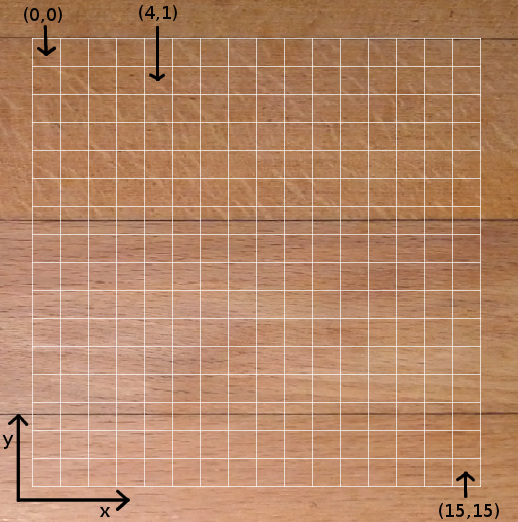
\includegraphics[scale = 0.25]{images/Spielbrett}
	\caption{Das Spielbrett.}
	\label{fig:Spielfeld}
\end{figure}
Das Spielbrett wird durch insgesamt \SpielFelderAnzahl\ Spielfelder gebildet, welche in einer 16x16 Matrix angeordnet sind.  Jedes Spielfeld besitzt eine eindeutige (x,y)-Koordinate. Die Nummerierung beginnt jeweils bei 0, wie in der Informatik üblich. (0,0) identifiziert demnach das Spielfeld ganz  oben links (siehe \autoref{fig:Spielfeld}).\\

\subsection{Die Spielsteine}

\begin{wrapfigure}[7]{r}{0.3\textwidth}
	\centering
	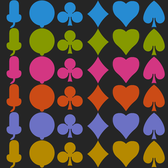
\includegraphics[scale = 0.45]{images/Spielsteine}
	%\caption{Die 36 möglichen Farbe-/Form-Kombinationen der Spielsteine}
	\caption{}
	\label{fig:Spielsteine}
\end{wrapfigure}
Ein Spielstein besitzt eine von sechs möglichen Farben und eine von sechs möglichen Formen. Die sechs Farben sind \emph{Blau},  \emph{Grün}, \emph{Magenta}, \emph{Orange}, \emph{Violett} und \emph{Gelb}. An Formen gibt es \emph{Eichel}, \emph{Schelle}, \emph{Kreuz}, \emph{Karo}, \emph{Herz} und \emph{Pik}.  Es existieren demnach 36 verschiedene Farb-/Form-Kombinationen (siehe \autoref{fig:Spielsteine}).\\
Von jeder Kombination gibt es genau drei Steine im Spiel, also insgesamt 108 Spielsteine.
\newpage

\subsection{Der Vorrat}
\begin{wrapfigure}[16]{r}{0.6 \textwidth}
	\centering
	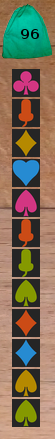
\includegraphics[scale = 0.5]{images/Vorratsbeutel}
	\caption{Der Vorrat}
	\label{fig:Vorrat}
\end{wrapfigure}
 Alle Spielsteine werden vor Beginn des Spiels gemischt und im Vorrat abgelegt. Dieser besteht aus Steinen im Beutel und bereits aufgedeckten Steinen (siehe \autoref{fig:Vorrat}). Die Zahl auf dem Beutel gibt die Anzahl, der sich noch im Vorrat befindenden Spielsteine an. Hierbei ist zu beachten, dass damit die Gesamtanzahl der Spielsteine im Vorrat gemeint ist, also sowohl die im Beutel, als auch die schon sichtbaren Spielsteine unterhalb des Beutels.\\
%\newpage
%\begin{figure}[h] \centering 
%	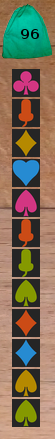
\includegraphics[scale = 0.7]{images/Vorratsbeutel}
%	\caption{Der Vorrat}
%	\label{fig:Vorrat2}
%\end{figure}

\section{Spielablauf}
	Zu Spielbeginn erhält jeder Spieler 6 Steine, die unterhalb des Spielbretts offen liegen, so dass der Gegner diese sehen kann. Im Vorrat befinden sich dann noch 96 Steine, von denen 12 aufgedeckt sind. Der rote Spieler beginnt.\\
 Jeder Spieler hat in seinem Zug zwei verschiedene Möglichkeiten. Entweder er legt einen oder mehrere Spielsteine auf dem Spielbrett aus, oder er tauscht zwischen 1 und 6 seiner Spielsteine gegen neue ein. Im ersten Zug müssen mindestens 2 Spielsteine ausgelegt werden. Ist dies nicht möglich, so muss der Spieler Steine tauschen.
 \newpage
	
\subsection{Spielsteine auslegen}
\begin{wrapfigure}[27]{r}{0.4\textwidth}
	\centering
	\begin{subfigures}
		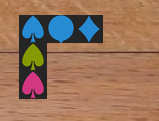
\includegraphics[scale = 0.7]{images/anlegen01}
		\caption{Zwei Reihen}
		\label{fig:Anlegen01}
		\vspace{8pt}
		
		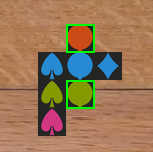
\includegraphics[scale = 0.7]{images/anlegen04}
		\caption{Anlegen von 2 Spielsteinen}
		\label{fig:Anlegen02}
		\vspace{8pt}
		
		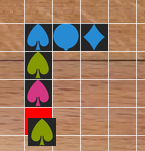
\includegraphics[scale = 0.7]{images/anlegen02}
		\caption{Ungültige Position. Die Reihe hat schon ein Pik derselben Farbe.}
		\label{fig:Anlegen03}
	\end{subfigures}	
\end{wrapfigure}
Beim Anlegen gelten folgende Regeln:
\begin{itemize}
\item Zwei oder mehr Steine, die horizontal oder vertikal unmittelbar nebeneinander liegen, bilden eine Reihe.
\item Eine Reihe besteht entweder aus Spielsteinen, welche die gleiche Farbe oder die gleiche Form besitzen.
\item In einer Reihe von gleichen Formen darf jede Farbe höchstens einmal vorkommen.
\item In einer Reihe von gleichen Farben darf jede Form höchstens einmal vorkommen.
\item Eine Reihe besteht somit aus maximal 6 Spielsteinen.
\item Ein Spielstein, der ausgelegt werden soll, muss immer an schon vorhandene Spielsteine angelegt werden. Ausnahme ist hier der als erstes ausgelegte Spielstein einer Partie. Dieser darf beliebig auf dem Spielbrett platziert werden.
\item Werden mehrere Steine in einem Zug ausgelegt, müssen diese sich in derselben Reihe befinden. Am Ende eines Zuges muss für alle auf dem Spielbrett unmittelbar horizontal oder vertikal nebeneinander liegenden Steine gelten, dass diese ausschließlich die zuvor beschriebenen Reihen bilden.
\end{itemize}


Um einen Stein anzulegen, klickt man auf diesen und zieht ihn auf das Spielbrett. Wenn eine mögliche Position angewählt wurde, wird das Spielfeld grün unterlegt. Ansonsten wird das Spielfeld rot unterlegt. Um alle bisher im Zug gelegten Steine zurückzuholen, klickt man auf den Button \emph{Steine zurücknehmen}. Um seinen Zug zu beenden und die momentan auf dem Spielbrett liegenden Steine fest anzulegen, klickt man auf den Button \emph{Steine legen}.\\
Nach dem Anlegen der Spielsteine werden die Steine des Spielers wieder auf 6 aufgefüllt. Die Steine, die dieser erhält, können in der Reihe unterhalb des Beutels eingesehen werden. Der Spielstein, welcher sich ganz unten befindet, ist der erste, den der Spieler erhält.
	 
\subsection{Spielsteine tauschen}
Ist ein Spieler mit seinen Steinen unzufrieden, kann er zwischen 1 und 6 Spielsteine gegen neue aus dem Vorrat tauschen. Kann ein Spieler keine Spielsteine anlegen, dann muss er Spielsteine tauschen.\\
Zum Tauschen klickt der Spieler die zu tauschenden Steine an. Diese werden dann durch einen grünen Rahmen umrandet. Um die Auswahl aufzuheben, kann man jeden Stein einzeln anklicken oder auf den Button \emph{Steine zurücknehmen} klicken. Sind Spielsteine zum Tausch ausgewählt, ist es nicht möglich, einen Stein auf dem Spielbrett auszulegen. Um den Tausch zu vollziehen, klickt der Spieler auf den Button \emph{Steine tauschen}.
 Er erhält dann die von ihm gewählte Anzahl von Spielsteinen aus den offen liegenden Spielsteinen und zwar von unten beginnend. Seine abgegebenen Steine werden zurück in den Beutel getan, welcher danach gemischt wird.
 Nach dem Tausch ist der Zug des Spielers beendet.
	
\subsection{Punkteverteilung}
\begin{wrapfigure}[10]{R}{0.4\textwidth}
	\centering	
		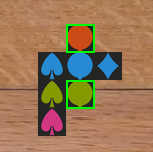
\includegraphics[scale = 0.7]{images/anlegen04}
		\caption{Für das Anlegen erhält der Spieler 5 Punkte.}
		\label{fig:Punkte1}	
\end{wrapfigure}
Beim Anlegen von Spielsteinen erhält man einen Punkt für jeden Stein, der sich in einer erweiterten Reihe befindet. Ein Stein wird doppelt gezählt, wenn er Teil von zwei Reihen ist (siehe \autoref{fig:Punkte1}).\\
Wenn man es schafft, eine Reihe von 6 Steinen zu erzeugen, bildet man ein \textbf{Sixpack}, für den es einen Bonus von 6 Punkten gibt (siehe \autoref{fig:PunkteSixpack}).\\
Das Tauschen von Spielsteinen bringt 2 Punkte, unabhängig davon, wie viele Steine getauscht werden.
\vspace{30pt}
\begin{figure}[h]
\centering
	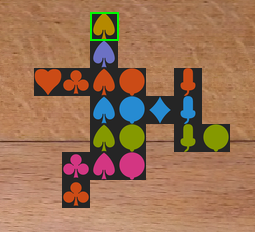
\includegraphics[scale = 0.6]{images/sixpack_legen}
		\caption{Das Anlegen des grün umrandeten Steines ergibt ein \emph{Sixpack}. (12 Punkte)}
		\label{fig:PunkteSixpack}	
\end{figure}

\newpage
	
\section{Ende des Spiels}
\label{sec:gameOver}
Das Spiel endet spätestens nach 20 Runden. Der Spiel endet vorher, sobald ein Spieler in einem Zug mehr Steine legt oder tauschen will, als sich noch im Vorrat befinden. Dieser Spieler erhält noch seine Punkte aus diesem Zug. Unmittelbar anschließend ist das Spiel beendet. Legt ein Spieler beispielsweise 4 Steine an, während sich nur noch 3 Steine im Vorrat befinden, so ist das Spiel nach diesem Zug vorbei.\\
Der Spieler mit den meisten Punkten gewinnt. Haben beide Spieler die gleiche Anzahl an Punkten, so gibt es ein Unentschieden.

\subsection{Spezialfall: Keine Züge mehr möglich}
Sollte der Fall eintreten, dass keine Spielsteine mehr angelegt werden können, so müssen die Spieler Steine tauschen, bis die maximale Rundenanzahl erreicht ist. Dieser Fall wird in der Praxis sehr selten vorkommen, kann aber beispielsweise auftreten, wenn ein 6x6-Quadrat gelegt wurde (siehe \autoref{fig:Spielsteine}).
\newpage
	
\section{Die graphische Benutzeroberfläche}
\subsection{Übersicht der graphischen Benutzeroberfläche}
\begin{figure}[h]
	\centering
	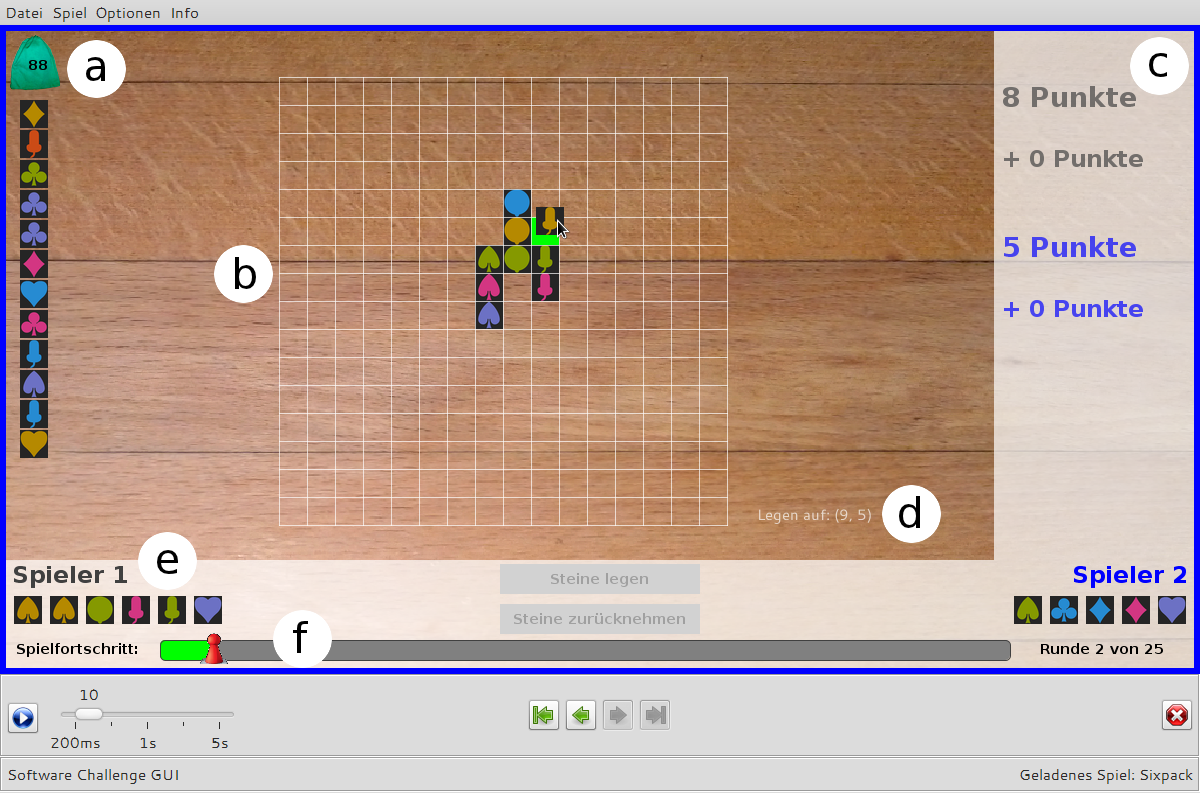
\includegraphics[width = \textwidth]{images/GUI}
	\caption{Die graphische Benutzeroberfläche}
\end{figure}
\begin{compactenum}[a)]
	\item Der Vorrat
	\item Das Spielbrett
	\item Punkteanzeige. Die Punkte des roten Spielers sind
	oben, die des blauen Spielers unten. Die Punkte des inaktiven Spielers werden immer grau angezeigt.
	\item Positionsanzeige
	\item Die Spielsteine von Spieler 1
	\item Spielfortschrittsanzeige
\end{compactenum}
	
\subsection{Das Einstellungsmenü}
	 \begin{figure}[h]
		\centering
		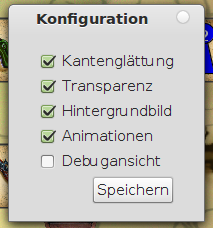
\includegraphics[scale=0.5]{images/configuration}
		\caption{Das Einstellungsmenü}
		\label{fig:Configuration}
	\end{figure}	
Ein Einstellungsmenü mit Darstellungsoptionen lässt
sich über die Leertaste anzeigen. Dazu muss das
Spielfeld den Tastaturfokus haben (erforderlichenfalls
vorher Mausklick auf das Spielfeld). Es stehen dort
folgende Einstellungen zur Verfügung:

\textbf{Kantenglättung} und \textbf{Transparenz} verbessern die Optik des
Spiels, sind jedoch rechenintensiv. Auf sehr langsamen Rechnern sollten sie daher
deaktiviert werden. \textbf{Hintergrundbild} ist zwar weniger rechenintensiv,
kann aber auch aus Gründen der Übersichtlichkeit deaktiviert werden.\\
\textbf{Animationen} legt fest, ob die Bewegungen der Spielsteine in
Wiederholungen und bei Computerspielern animiert werden sollen.\\
Die \textbf{Debugansicht} verkleinert die Punkteanzeige in der Seitenleiste
etwas und zeigt unterhalb Debug-Hilfestellungen zu einzelnen Zügen an. Diese
Hilfestellungen sind Texte, die ein Computerspieler einem Zug beifügen kann, den er
an den Spielserver sendet.
	
\end{document}
